\documentclass{beamer}
\usepackage{hyperref}
\usepackage{subfig}  %% To include subfigures
\usepackage{media9} % 
\usepackage{ragged2e}  % Allow justification
\usepackage{url}
\usepackage[margin=20pt,font=small,labelfont=bf,labelsep=period]{caption}

\hypersetup{pdfstartview={Fit}, bookmarks=True, pdftitle={Wave Propagation Lectures},
            pdfauthor={Nicolas Guarin-Zapata}, pdfsubject={Lectures},
            pdfkeywords={Waves, Elasticity, Numerical Methods}}  % Configure hyperref

%--- New commands ----%
\newcommand{\footref}[1]{\textsuperscript{\ref{#1}}}
\newcommand{\pardiff}[2]{\frac{\partial #1}{\partial #2}}
\newcommand{\pardiffd}[2]{\frac{\partial^2 #1}{\partial #2^2}}
%---------------------%

%\usefonttheme[onlymath]{serif}  % Make equations to be in serif fonts
\usefonttheme{serif}  % Make equations to be in serif fonts

\begin{document}


%title
\title[Wave propagation in solids] % (optional, only for long titles)
{Wave propagation:}
\subtitle{Numerical tools}
\author[Guarin-Zapata, Nicolas] % (optional, for multiple authors)
{Nicol\'as Guar\'in Zapata\\ \texttt{\small nguarin@purdue.edu}\\
{\tiny Slides available at: \url{https://github.com/nicoguaro/CE597-slides}}}
\institute{Civil Engineering Department\\
  Purdue University}
\date{\today}
\subject{Wave propagation}

% Title page
\frame{\titlepage}

% Outline
\begin{frame}
	\frametitle{Outline}
	\tableofcontents
\end{frame}
%

%  Relations between elastic constants
\section{Relations between elastic constants}
\begin{frame}[shrink=50]
\frametitle{Relations between elastic constants}
\centering

\vspace{3cm}
\begin{table}[h]
\centering %
\begin{tabular}{|c|c|c|c|c|c|c|c|c|c|c|}
\hline 
 & $(K,E)$  & $(K,\lambda)$  & $(K,G)$  & $(K,\nu)$  & $(E,G)$  & $(E,\nu)$  & $(\nu,G)$  & $(\nu,\lambda)$  & $(G,\lambda)$  & $(G,M)$ \\
\hline 
$K=$  & $K$  & $K$  & $K$  & $K$  & $\frac{EG}{3(3G-E)}$  & $\frac{E}{3(1-2\nu)}$  & $\lambda+\frac{2G}{3}$  & $\frac{\lambda(1+\nu)}{3(1-2\nu)}$  & $\frac{2G(1+\nu)}{3(1-2\nu)}$  & $M-\frac{4G}{3}$ \\
\hline 
$E=$  & $E$  & $\frac{9K(K-\lambda)}{3K-\lambda}$  & $\frac{9KG}{2K+G}$  & $3K(1-2\nu)$  & $E$  & $E$  & $\frac{G(3\lambda+2G)}{\lambda+G}$  & $\frac{\lambda(1+\nu)(1-2\nu)}{\nu}$  & $2G(1+\nu)$  & $\frac{G(3-M-4G)}{M-2G}$ \\
\hline 
$\lambda=$  & $\frac{3K(3KE)}{9K-E}$  & $\lambda$  & $K-\frac{2G}{3}$  & $\frac{3K\nu}{1+\nu}$  & $\frac{G(E-2G)}{EG-E}$  & $\frac{E\nu}{(1+\nu)(1-2\nu)}$  & $\lambda$  & $\lambda$  & $\frac{2G\nu}{1-2\nu}$  & $M-2G$ \\
\hline 
$G=$  & $\frac{3KE}{9K-E}$  & $\frac{3(K-\lambda)}{2}$  & $G$  & $\frac{3K(1-2\nu)}{2(1+\nu)}$  & $G$  & $\frac{E}{2(1+\nu)}$  & $G$  & $\frac{\lambda(1-2\nu)}{2\nu}$  & $G$  & $G$ \\
\hline 
$\nu=$  & $\frac{3K-E}{6K}$  & $\frac{\lambda}{3K-\lambda}$  & $\frac{3K-2G}{2(3K+G)}$  & $\nu$  & $\frac{E}{2G}-1$  & $\nu$  & $\frac{\lambda}{2(\lambda+G)}$  & $\nu$  & $\nu$  & $\frac{M-2G}{2(M-G)}$ \\
\hline 
$M=$  & $\frac{3K(3K+E)}{9K-E}$  & $3K-2\lambda$  & $K+\frac{4G}{3}$  & $\frac{3K(1-\nu)}{1+\nu}$  & $\frac{G(4G-E)}{3G-E}$  & $\frac{E(1-\nu)}{(1+\nu)(1-2\nu)}$  & $\lambda+2G$  & $\frac{\lambda(1-\nu)}{\nu}$  & $\frac{2G(1-\nu)}{1-2\nu}$  & $M$ \\
\hline 
\end{tabular}
\end{table}

{\large $K$: Bulk modulus, $\lambda$: Lam\'e's first parameter, $E$: Young's
modulus, $G$: Shear modulus, $\nu$: Poisson's ratio, $M$: P-wave
modulus.}
\end{frame}

% Elastodynamics equations
\section{Elastodynamic wave equations}
\subsection{Navier-Cauchy Equations}
\begin{frame}
\frametitle{Navier-Cauchy Equations}
The Navier-Cauchy equations read
\begin{equation}
\rho{ \pardiffd{\bold{u}}{t}} = \bold{f} + ( \lambda + 2G)\nabla(\nabla \cdot \bold{u}) - G\nabla \times (\nabla \times \bold{u}) \enspace ,
\label{eq:navierVec}
\end{equation}
or, rearranging the constants
\begin{equation}
 \pardiffd{\bold{u}}{t} = \bold{f} + \alpha^2\nabla(\nabla \cdot \bold{u}) - \beta^2\nabla \times (\nabla \times \bold{u}) \enspace ,
\label{eq:navierVec2}
\end{equation}
being $\alpha$ the speed of the P-wave and $\beta$ the speed of the S-wave. According to this, our problem just depends on two material properties, the two wave speeds.

\end{frame}

% Relations for elastic wave speeds
\subsection{Relations for elastic wave speeds}
\begin{frame}[allowframebreaks]
\frametitle{Relations for elastic wave speeds}
The P-wave is a dilatational wave with speed $\alpha$ given by 
\begin{align*}
 & \alpha^{2}=\frac{\lambda+2G}{\rho},\qquad\alpha^{2}=\frac{G(1-\nu)}{\rho},\\
 & \alpha^{2}=\frac{M}{\rho},\qquad\alpha^{2}=\frac{E(1-\nu)}{(1+\nu)(1-2\nu)\rho},\\
 & \alpha^{2}=\frac{2\beta^{2}(1-\nu)}{1-2\nu}.
\end{align*}
 The S-wave is a distorsional wave with speed $\beta$ given by 
\begin{align*}
 & \beta^{2}=\frac{G}{\rho}\\
 & \beta^{2}=\frac{E}{2(1+\nu)\rho},\\
 & \beta^{2}=\frac{\alpha^{2}(1-2\nu)}{2(1-\nu)}.
\end{align*}
 Some particular values for the ratio 
\[
\frac{\alpha^{2}}{\beta^{2}}=\frac{2(1-\nu)}{1-2\nu}
\]
 are 
\begin{align*}
 & \frac{\alpha^{2}}{\beta^{2}}=\frac{4}{3}\quad\mbox{for }\nu=-1\enspace,\\
 & \frac{\alpha^{2}}{\beta^{2}}=2\quad\mbox{for }\nu=0\enspace,\\
 & \frac{\alpha^{2}}{\beta^{2}}=4\quad\mbox{for }\nu=\frac{1}{3}\enspace,\\
 & \frac{\alpha^{2}}{\beta^{2}}\rightarrow\infty\quad\mbox{when }\nu\rightarrow\frac{1}{2}\enspace.
\end{align*}
\end{frame}

\subsection{Ashby chart: $E$ vs. $\rho$}
\begin{frame}{Ashby chart: $E$ vs. $\rho$}
\begin{figure}
\includegraphics[height=6cm]{img/E_vs_density-vector.pdf} 
\caption{Ashby chart for Young Modulus vs density. The lines show the sound speed, that is the speed for a wave in a rod made of this
material.  This value is between the longitudinal and shear wave speeds for Poisson ratios in (-0.5,0.5). \cite{ashby2005}}
\end{figure}
\end{frame}

% Solution
\section{Solution}
\subsection{Time domain vs. Frequency domain}
\begin{frame}[allowframebreaks]{Time domain vs. Frequency domain}
If we are interested in waves, we are interested in dynamic behavior. To find the solutions to the (linear) equations  we can use one of two approaches:
\begin{itemize}
\item \textbf{Time domain,} in this case the equations are solved directly.
\item \textbf{Frequency domain,} the solution is expressed as the superposition (sum) of individual waves with different frequencies. This means that the solutions to the equation (and forces) are of the form
\[\bold{u} = \bold{U} \exp(-i\omega t), \text{and } \bold{f} = \bold{F} \exp(-i\omega t)\]
substituting in the original equation we obtain
\begin{equation}
 \alpha^2\nabla(\nabla \cdot \bold{U}) - \beta^2\nabla \times (\nabla \times \bold{U})  + \bold{F} = -\omega^2\bold{U} \enspace ,
\label{eq:navier_freq}
\end{equation}

\pagebreak
Then, we transformed the problem of solving a dynamic equation into solving a set of steady-state problems. For every waveform there is an equivalent function in the frequency domain, i.e., its spectrum.\footnote{This can be formally defined using the Fourier transform, and computed numerically (efficiently) using the FFT algorithm.}
\end{itemize}

\begin{figure}[h]
\centering
\subfloat[Ricker pulse.]{\includegraphics[width=0.4\textwidth]{img/ricker_pulse.pdf}}\qquad
\subfloat[Ricker pulse spectrum.]{\includegraphics[width=0.4\textwidth]{img/ricker_area=2.pdf}}
\caption{Ricker pulse and its spectrum.}

\end{figure}
\end{frame}

\subsection{Numerical methods for waves in solids}
\begin{frame}
\frametitle{Numerical methods for waves in solids}
Exact solutions for the Navier-Cauchy equations are more an exception than the norm. So, we need methods to approximate the solutions (that's the role of numerical methods in general). A rough classification of the methods used in elastodynamics is:
\begin{itemize}
\item Spectral/Pseudo-spectral methods
\item Domain Discretization methods
\begin{itemize}
\item Finite Difference Methods (FDM)
\item Finite Volume Methods (FVM)
\item Finite Element Methods (FEM)
\item Boundary Element Methods (BEM)
\end{itemize}
\end{itemize}
\end{frame}

\subsubsection{Spectral/Pseudo-spectral methods}
\begin{frame}{Spectral/Pseudo-spectral method}
In this class of methods we expand the functions of interest in terms of a (orthogonal) basis \cite{wiki:pseudo_spectral}, i.e.
\[\bold{U}(\bold{x}) = \sum\limits_{n=1}^N c_n h_n(\bold{x}) \enspace ,\]
e.g., we can use a combination of sine functions
\[\bold{U}(\bold{x}) = \sum\limits_{n=1}^N c_n \sin(k_n\bold{x}) \enspace .\]
This methods produce very accurate solutions and present good convergence rates, but are difficult to apply for complex geometries.
\end{frame}

\subsubsection{Domain discretization methods}
\begin{frame}{Domain dizcretization methods}
In this set of methods the domain of interest is subdivided (discretized) to obtain a system of linear/algebraic equations. After applying the discretization process we end up with a system like
\[[K]\lbrace \bold{u}\rbrace + [M]\lbrace \bold{a}\rbrace = \lbrace \bold{f}\rbrace \enspace ,\]
in the time domain, and
\[[K]\lbrace \bold{U}\rbrace - \omega^2 [M]\lbrace \bold{U}\rbrace = \lbrace \bold{F}\rbrace \enspace ,\]
in the frequency domain. In both equations $[K]$,  and $[M]$ are termed stiffness and mass matrices.

\end{frame}

\subsubsection{Finite Difference Methods}
\begin{frame}{Finite Difference Methods}
In FDM the domain is (commonly) decomposed in rectangular regions where the function is constant \cite{wiki:FDM}. The differential equation is approximated with difference equations, e.g.
\[\pardiff{u}{x} \approx \frac{u(x + \Delta x) - u(x)}{h}\]
\begin{figure}
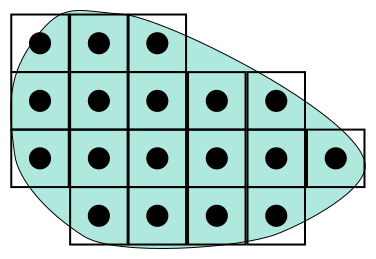
\includegraphics[height=4cm]{img/FDM.pdf} 
\caption{Schematic domain discretized in rectangular cells.}
\end{figure}
\end{frame}

\subsubsection{Finite Volume Methods}
\begin{frame}{Finite Volume Methods}
In FVM the geometry is decomposed into regions, denoted as \emph{Finite volumes}. Some quantities are evaluated (as fluxes) at the interface between neighboring \emph{finite volumes}, these methods are conservative. This method is more used in CFD, but it is also popular for wave propagation.\footnote{See for example Clawpack: \url{http://depts.washington.edu/clawpack/}.}
\begin{figure}
\includegraphics[height=4cm]{img/FVM.pdf} 
\caption{A finite volume and its surfaces.}
\end{figure}

\end{frame}

\subsubsection{Finite Element Methods}
\begin{frame}{Finite Element Methods}
The FEM is a method that is based on variational principles. It approximates a function in a finite set of points over the domain. To populate the matrices, the domain is split in several subregion called \emph{elements}.

\textcolor{blue}{But I'm sure you are going to talk more about this in the rest of the course}
\begin{figure}
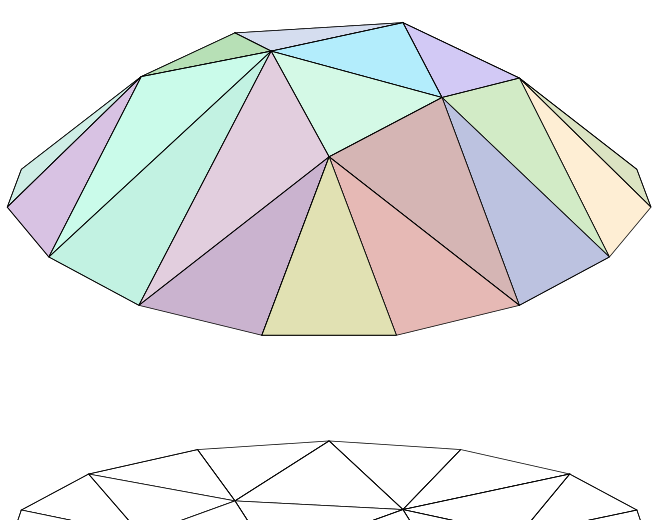
\includegraphics[height=4cm]{img/Piecewise_linear_function2D.pdf} 
\caption{A piecewise function represented via {finite elements}. From: \url{https://commons.wikimedia.org/wiki/File:Piecewise_linear_function2D.svg}}
\end{figure}

\end{frame}

\subsubsection{Boundary Element Methods}
\begin{frame}{Boundary Element Methods}
The BEM is similar in formulation to the FEM. The main difference lies in the dimensionality of the mesh, since it only requires the discretization of the contour. This method is really popular in fracture mechanics and wave propagation, the latter due to the capability of represent infinite domains.
\begin{figure}
\includegraphics[height=4cm]{img/BEM.pdf} 
\caption{2D domain and the discretization of its contour using Boundary Elements.}
\end{figure}

\end{frame}

\subsection{CFL Condition}
\begin{frame}[allowframebreaks]
\frametitle{CFL Condition}
\justifying
The Courant-Friedrichs-Lewy condition (CFL condition) is a necessary
condition for convergence while solving PDEs by the method of finite
differences \cite{CFL}. It arises when explicit time-marching schemes are used.

The criterion could be stated as 
\begin{align*}
C=v_{x}\frac{\Delta t}{\Delta x}\leq C_{max}\qquad\mbox{in 1D}\enspace;\\
C=v_{x}\frac{\Delta t}{\Delta x}+v_{y}\frac{\Delta t}{\Delta y}\leq C_{max}\qquad\mbox{in 2D}\enspace;\\
C=v_{x}\frac{\Delta t}{\Delta x}+v_{y}\frac{\Delta t}{\Delta y}+v_{z}\frac{\Delta t}{\Delta z}\leq C_{max}\qquad\mbox{in 3D}\enspace;
\end{align*}
 Where $v_{x_{i}}$ is the wave speed in the
$x_{i}$ direction, $\Delta x_{i}$ is the minimum spatial discretization
in $x_{i}$ direction, $\Delta t$ is the time step and $C_{max}$
is the maximum allowable value for $C$, which depends on the time
discretization scheme but should be less than 1.

A graphical representation of the criterion is given in Figure \ref{fig:CFL}. Intuitively, we can think about the CFL condition as a limit in the speed for transferring information from one node to its neighbors; this \emph{speed} should be less than the speed for propagation of phenomena in the wave. 
\begin{figure}
\centering
\includegraphics[height=4cm]{img/CFLcondition.png} 
\caption{Graphic representation of the CFL condition in 1D. \textit{L.A. Barba et al. Practical Numerical Methods with Python, 2014.}}\label{fig:CFL}
\end{figure}

In elastodynamics, and using the the FEM, the criterion could be re-stated as 
\begin{align*}
C\leq\alpha\frac{\Delta t}{h}\leq C_{max}\qquad\mbox{in 1D}\enspace;\\
C\leq2\alpha\frac{\Delta t}{h}\leq C_{max}\qquad\mbox{in 2D}\enspace;\\
C\leq3\alpha\frac{\Delta t}{h}\leq C_{max}\qquad\mbox{in 3D}\enspace;
\end{align*}
 where $\alpha$ is the speed for the P-wave and $h$ is the
minimum distance between consecutive nodes. This give us the maximum
allowable timestep as 
\begin{align}
\Delta t\leq C_{max}\frac{h}{\alpha}\qquad\mbox{in 1D}\enspace;\\
\Delta t\leq\frac{C_{max}}{2}\frac{h}{\alpha}\qquad\mbox{in 2D}\enspace;\\
\Delta t\leq\frac{C_{max}}{3}\frac{h}{\alpha}\qquad\mbox{in 3D}\enspace.
\end{align}
\end{frame}

\subsection{Nyquist-Shannon sampling criterion}
\begin{frame}[allowframebreaks]
\frametitle{Nyquist-Shannon sampling criterion}
\justifying
The Nyquist--Shannon sampling theorem is a fundamental
result in the field of information theory, in particular telecommunications and signal processing. Sampling is the process of converting a signal (for example, a function of continuous time or space) into a numeric sequence (a function of discrete time or space).
\begin{figure}
\centering
\includegraphics[height=2cm]{img/{CPT-sound-nyquist-thereom-1.5percycle}.pdf} 
\caption{The samples of several different sine waves can be identical, when at least one of them is at a frequency above half the sample rate. From: \url{https://commons.wikimedia.org/wiki/File:CPT-sound-nyquist-thereom-1.5percycle.svg}}
\end{figure}

Shannon's version of the theorem states \cite{Shannon}:

\begin{quote}
If a function $x(t)$ contains no frequencies higher than $B$ hertz,
it is completely determined by giving its ordinates at a series of
points spaced $1/(2B)$ seconds apart. 
\end{quote}
This theorem implies for us in the numerical simulation of wave propagation
that 
\[
h\leq\frac{\lambda}{2}\enspace,
\]
 where $h$ is the maximum distance between consecutive nodes and
$\lambda$ is the shortest wavelength that want to be sampled. So,
the selection of $h$ is commonly 
\[
h=\frac{\lambda}{k}\enspace,
\]
 where $k>2$ is a factor that depends on the numerical method. For
finite element methods $k$ is commonly 10.
\end{frame}

\begin{frame}[allowframebreaks]{References}
\def\newblock{}
\bibliographystyle{plain}
\begin{thebibliography}{1}

\bibitem{book:arfken} George B. Arfken \& Hans. J. Weber. Mathematical Methods for Physicists. Elsevier Academic Press, 6th Edition, San Diego, 2005.

\bibitem{ashby2005} Ashby, Michael F. ``Materials
selection in mechanical design." MRS BULLETIN 30 (2005): 995.

\bibitem{CFL} Courant, R.; Friedrichs, K.; Lewy, H. (1928), \emph{\"Uber
die partiellen Differenzengleichungen der mathematischen Physik} (in
German), Mathematische Annalen 100 (1): 32--74.

\bibitem{Shannon} C. E. Shannon, \emph{Communication in the presence
of noise}, Proc. Institute of Radio Engineers, vol. 37, no. 1, pp.
10--21, Jan. 1949. Reprint as classic paper in: Proc. IEEE, vol. 86,
no. 2, (Feb. 1998).

\bibitem{book:waves-rays} Michael A. Slawinski. Waves and rays in Elastic Continua. Second Edition, 2007.
 
\bibitem{wiki:FDM} Finite difference method. (2014, April 29). In Wikipedia, The Free Encyclopedia. Retrieved 00:11, September 25, 2014, from \url{http://en.wikipedia.org/w/index.php?title=Finite_difference_method&oldid=606345831}

\bibitem{wiki:FVM} Finite volume method. (2014, April 22). In Wikipedia, The Free Encyclopedia. Retrieved 00:44, September 25, 2014, from \url{http://en.wikipedia.org/w/index.php?title=Finite_volume_method&oldid=605282055}
 
\bibitem{wiki:ondas} Wikipedia community. Onda (f\'isica) [on line]. Wikipedia, La enciclopedia libre, 2010 ; 22 November 2010.

\bibitem{wiki:pseudo_spectral} Pseudo-spectral method. (2014, March 14). In Wikipedia, The Free Encyclopedia. Retrieved 23:12, September 24, 2014, from \url{http://en.wikipedia.org/w/index.php?title=Pseudo-spectral_method&oldid=599542680}

\end{thebibliography}

\end{frame}



\end{document}

